\newpage

\section{Edge-to-Cloud Integration via MQTT}

\subsection{Theoretical Background}
To ensure low-latency, bidirectional communication between the central processing node (PC) and the ESP32 firmware, the H.E.R.A system employs the MQTT (Message Queuing Telemetry Transport) protocol. MQTT operates on a lightweight publish-subscribe model managed by a central broker. \\

In this architecture, both the ESP32 edge device and the backend PC act as MQTT clients. They do not communicate directly; instead, they publish messages to specific "topics" and subscribe to topics they need to monitor. The broker is responsible for routing these messages efficiently. \\

MQTT was selected over traditional request-response protocols like HTTP due to several key advantages for IoT applications:
\begin{itemize}
    \item \textbf{Lightweight and Low Bandwidth:} MQTT minimizes packet overhead, making it highly efficient for constrained embedded devices sending frequent payloads.
    \item \textbf{Asynchronous Communication:} The publish-subscribe model decouples the sender and receiver, allowing the ESP32 to push sensor data continuously without waiting for the PC to request it.
    \item \textbf{Low Latency:} Persistent TCP connections enable near-instantaneous transmission of execution commands from the PC down to the edge actuators.
\end{itemize}

\subsection{Firmware Implementation (Edge Node)}
At the edge layer, the ESP32 firmware manages the physical hardware and acts as the primary data publisher. Operating within a dedicated FreeRTOS task, the firmware handles two main MQTT operations:

\begin{itemize}
    \item \textbf{Telemetry Publishing:} Every 5 seconds, the ESP32 aggregates real-time environmental data and actuator states into a comprehensive JSON payload. This payload is published to the \texttt{v1/devices/me/telemetry} topic. The structured data is categorized into three main objects:
    \begin{itemize}
        \item \texttt{network}: Diagnostics including Wi-Fi RSSI, local IP, MQTT connection status, and device uptime.
        \item \texttt{sensors}: Real-time readings from the DHT20 (temperature, humidity), light sensor, and MQ-2 gas sensor.
        \item \texttt{devices}: Current operational states (status, brightness, color, voltage) of actuators such as the main LED, NeoPixels, WS2812 strip, relay, and mini fan.
    \end{itemize}

    \begin{lstlisting}[language=json, caption={Sample Telemetry JSON Payload published by ESP32}, label={lst:mqtt_telemetry}]
        {
        "network": {
            "wifi_connected": true,
            "wifi_rssi": -40,
            "wifi_ip": "127.0.0.1",
            "mqtt_connected": true,
            "uptime_ms": 75032
        },
        "devices": {
            "neo_led": {
            "status": false,
            "brightness": 60,
            "color": "#0000FF",
            "voltage": 0.0
            }
        },
        "sensors": {
            "dht20": {
            "temperature": 28.56,
            "humidity": 35.29,
            "voltage": 3.3
            }
        }
        }
    \end{lstlisting}
    \item \textbf{Command Execution:} The firmware continuously subscribes to the RPC (Remote Procedure Call) topic \texttt{v1/devices/me/rpc/request/+}. Upon receiving a command, it parses the payload to safely toggle physical devices or adjust parameters (like LED brightness or fan speed), then immediately returns confirmation responses.
\end{itemize}

\subsection{Backend Implementation (PC Node)}
On the backend PC, communication is handled by a dedicated Python module (\texttt{mqtt\_manager.py}). This script serves as the primary bridge between the data storage, the AI pipeline, and the hardware edge.

\begin{itemize}
    \item \textbf{Telemetry Ingestion \& Logging:} The backend subscribes to the telemetry topic. Upon receiving the 5-second JSON updates from the ESP32, it parses the multi-modal data and directly inserts it into the database (e.g., logging environmental records associated with specific user sessions).
    \item \textbf{Interactive CLI Interface:} For manual oversight and direct hardware control, the backend runs a terminal-based "H.E.R.A. CONTROL CENTER". This interactive menu allows developers or administrators to input numeric options (0-18) to trigger Lighting Controls, Device Controls, or System Monitoring functions.
    \item \textbf{RPC Payload Generation:} When an action is initiated via the CLI, the backend constructs a structured RPC request. For instance, selecting the option to "Set NeoPixel Brightness" and inputting a value of 60 prompts the backend to generate the payload \texttt{\{"method": "setStripBrightness", "params": 60\}}. This is then published to a dynamic request topic (e.g., \texttt{v1/devices/me/rpc/request/2908}), ensuring the ESP32 executes the command accurately and responsively.
\end{itemize}

\begin{figure}[htbp]
    \centering
    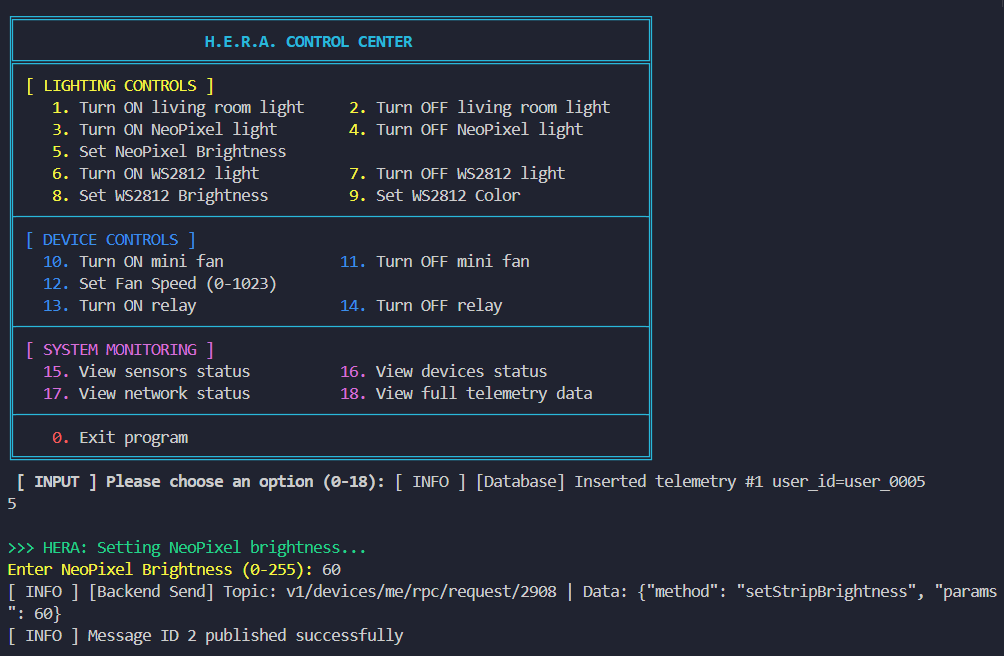
\includegraphics[width=0.9\textwidth]{image/mqtt_terminal.png}
    \caption{H.E.R.A. Control Center CLI interface demonstrating an RPC request for NeoPixel brightness adjustment.}
    \label{fig:cli_interface}
\end{figure}